%\addcontentsline{toc}{chapter}{SPRING}
\chapter{SPRING}
%\stepcounter{chapter}
El entorno de trabajo de Spring es popular y ampliamente usado entorno de trabajo de Java para construir aplicaciones web y de empresa. Su eje es la inyección de dependencias que provee flexibilidad para configurar de múltiple maneras, tales como XML, Commentarios, y configuraciones java. El entorno de trabajo Spring creció respondiendo a modernas necesidades de empresas como la seguridad, soporte para almacenamientos NoSql, manejo de GrandesDatos, proceso de lotes, integración con otros sistemas, etc. 

El entorno de trabajo Spring es flexible, tiene capacidad y fácil de uso transacciones de base de datos. simplifica la integración con otros entornos de trabajo, tiene una tecnología de punta para construir aplicaciones web en Modelo Vista Controlador. 
\section{Spring Boot}
Spring Boot es un entorno de trabajo que ayuda a desarrollar aplicaciones basados en Spring de forma fácil y rápida. Sus característica son:
\begin{itemize}
\item Iniciador de Spring Boot
\item Auto configuración
\item Manejo de configuración elegante
\item Actuador Spring Boot
\item Soporte de contenidos servlet y fácil de usar integrado
\end{itemize}

Spring Boot configura los componentes de la aplicación de forma automática, pero permitiendo invalidad los por defectos si requiere. 
Los pasos son:
\begin{enumerate}
\item Crear proyectos de Spring Boot basado en Maven y configurar las dependencias en el archivo \textit{pom.xml}
\item Configurar los recursos de datos/propiedades JPA en src/main/resources/aplication.properties.
\item Crear una entidad JPA llamada Usuario.java, una interfaz de repositorio de dato JPA Spring llamada RepositorioUsuario.java, y un controlador llamado HomeController.java
\item Crear un la vista para mostrar la lista de usuarios. 
\item Crea una una ClasePuntoEntrada Aplicacion.java con el método principal
\item Ejecutar la aplicación.java y dirigirse en el navegador al localhost:8080/
\end{enumerate}
Explicamos lo que está pasando:
\section{Fásil manejo de dependencias}
La dependencia llamada spring-boot-starter-*. este jala todas las librerías comunes al desarrollar aplicaciones Spring MVC tales como: spring-webmvc, jackson-json, validation-api, y tomcat. 
\section{Autoconfiguración}
Es su @EnableAutoConfiguration anote. 
\section{Soporte integrado de contenedor de servlet}
Se crea un clase simple comentado con (@SpringAplication), 

\subsection{Spring Initializr}
Para comenzar con el proyecto de Spring Boot se deber ir a la página \url{https://start.spring.io/}, configurar y pulsar generar. 
\begin{figure}[h]
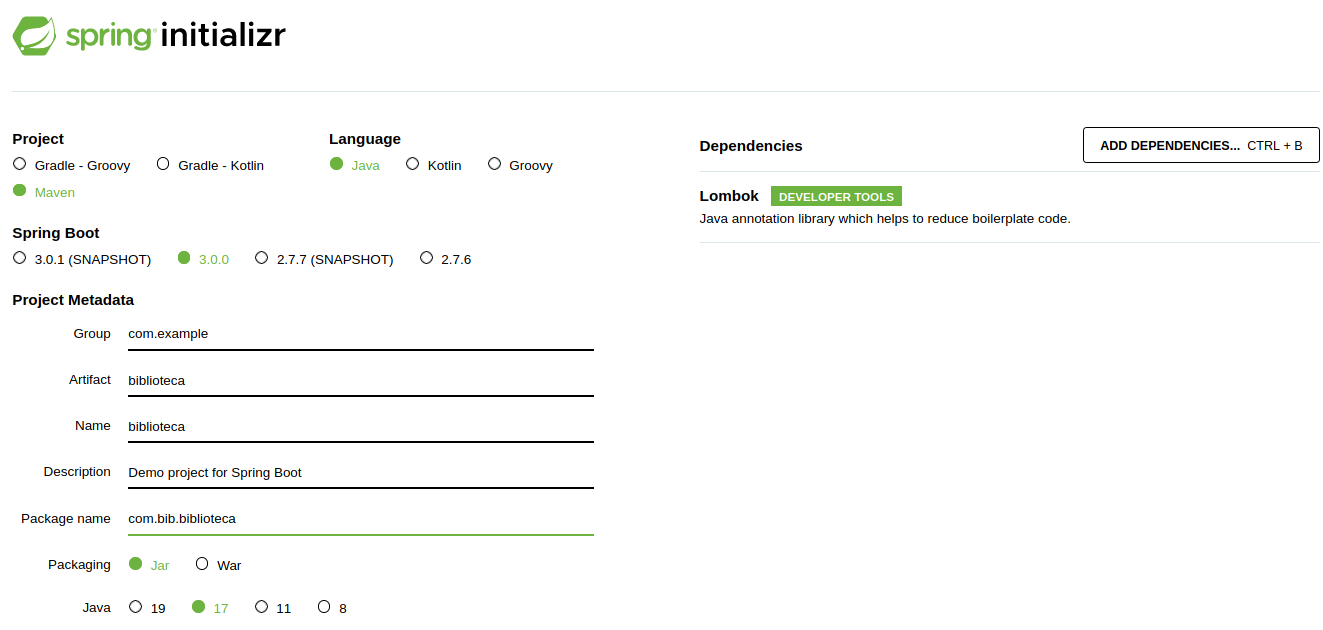
\includegraphics[scale=0.5]{images/spring1}
\caption{La configuración al iniciar un proyecto Spring Boot}
\end{figure}
Se verifica java para configurar. 
\begin{verbatim}
tomas@debian:~$ java --version
openjdk 17.0.4 2022-07-19
OpenJDK Runtime Environment (build 17.0.4+8-Debian-1deb11u1)
OpenJDK 64-Bit Server VM (build 17.0.4+8-Debian-1deb11u1, mixed mode, sharing)
\end{verbatim}

\section{Herramientas de desarrollo}



